\chapter{Tecnologías para la implementación del sistema}

Un nodo colector de datos debe considerar distintas interfaces de comunicación entre la WSN y el exterior que se escogen en base al propósito y las necesidades de la aplicación, ver figura \ref{fig:colector_datos}. Por un lado, diversos estándares han sido propuestos para formar WSN, cada uno implementando un conjunto de funciones y protocolos que buscan explotar características particulares de cada aplicación\cite{yick:wsn_survey}.

\begin{figure}
	\centering
	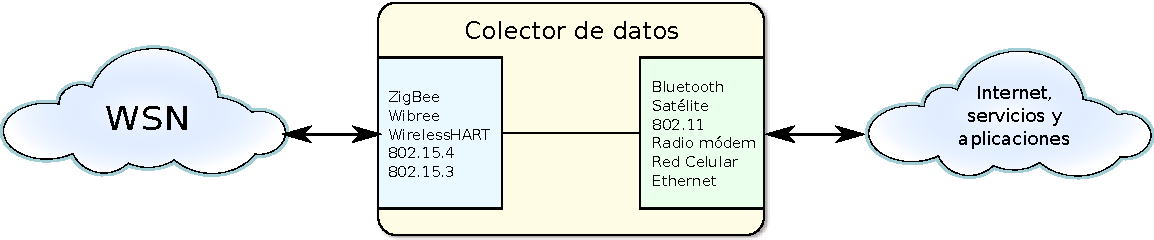
\includegraphics[scale=0.8]{capitulo_2_imgs/colector_de_datos.pdf}
	\caption{Tecnolog\'ias para la implementaci\'on de un nodo colector de datos.}
	\label{fig:colector_datos}
\end{figure}

Por otra parte, la elección de la tecnología para comunicar una WSN hacia el exterior depende de sus condiciones de operación. Por ejemplo, sensores instalados en entornos urbanos contarán con mayor disponibilidad de servicios de comunicación como acceso a redes inalámbricas locales, conexión mediante cable Ethernet o conexión directa con una computadora por un puerto USB. Mientras que en el caso contrario, en zonas remotas y de difícil acceso es necesario enlaces con mayor cobertura y autonomía como enlaces de radio y comunicación satelital. 

En la aplicación que se considera en este trabajo se emplean los estándares IEEE 802.15.4 y ZigBee para formar la WSN mientras que para la comunicación remota desde la WSN hacia la estación base se utiliza GSM/GPRS como medio de transporte. En el presente capítulo se mencionan las consideraciones que determinan las tecnologías utilizadas en esta aplicación, así como un conjunto de conceptos que es necesario definir para desarrollar el dispositivo propuesto. 

\section{El grupo de est\'andares IEEE 802.15}

Dentro del grupo IEEE 802.15 se han definido diversos estándares para la implementación de redes inalámbricas de área personal (\textit{Wireless Personal Area Networks}, WPAN). Por ejemplo, en IEEE 802.15.1 se establecen las normas de comunicación para dispositivos portátiles de corto alcance y en IEEE 802.15.3 se definen los métodos para establecer enlaces inalámbricos con un amplio ancho de banda para aplicaciones multimedia. Asi mismo, el estándar 802.15.4 define la comunicación a bajas velocidades de transmisión orientado a aplicaciones de monitoreo y control\cite{comparative:wireless_protocols}. 

El estándar IEEE 802.15.4 define los métodos y esquemas para el desarrollo de WSN y se utiliza como base para definir otros estándares y tecnologías complementarias. En la tabla \ref{tabla:estandares} se muestra una comparación de estándares para WSN. \textit{Bluetooth Low Energy}\cite{bluetooth:low_energy}, por ejemplo, es una modificación al estándar IEEE 802.15.1 (\textit{Bluetooth}) que permite enlaces inalámbricos de hasta 1 Mbps con un significativo ahorro de energía respecto a su antecesor. \textit{UWB} es una extensión a IEEE 802.15.3 que ofrece enlaces inalámbricos de hasta 200 Mbps con alcance de 10 metros con un consumo de energía entre 100 mW y 250 mW.  

Los estándares complementarios a IEEE 802.15.4 agregan funcionalidades de red, seguridad, entre otras. Por ejemplo, \textit{WirelessHART}\cite{estandar:wirelesshart} ofrece una implementación del protocolo de monitoreo industrial HART con comunicación inalámbrica de bajo consumo de energía, \textit{6LoWPAN}\cite{estandar:6lowpan} ofrece comunicación con protocolos IP entre dispositivos para aplicaciones donde se requiere conectividad hacia Internet, por último ZigBee provee comunicación inalámbrica optimizando el consumo de energía permitiendo la autonomía de los dispositivos durante años. De estos estándares, ZigBee es el más utilizado para la mayoría de las aplicaciones de WSN.  

Para el monitoreo de deslizamientos de laderas se requiere desplegar sensores en zonas alejadas o de difícil acceso, donde la supervisión humana periódica puede ser peligrosa, la frecuencia de ocurrencia del fenómeno a observar es desconocida y existe la posibilidad de pérdida del equipo; estos requerimientos de operación son cubiertos por ZigBee. De esta forma, dispositivos de bajo costo pueden monitorear las variables involucradas en el deslizamiento de laderas de manera autónoma durante años utilizando baterías como fuente de energía. 

\begin{table}
	\begin{center}
		
		\caption{Comparación de estándares para WSN}
		\label{tabla:estandares}
		\small
		\begin{tabular}{p{2.1cm}p{4cm}p{3.2cm}p{3.2cm}}
		
		\toprule
		\textbf{Estándar} & \textbf{Características} & \textbf{Ventajas} & \textbf{Desventajas}\\
		\midrule
		Bluetooth Low Energy & Basado en Bluetooth, velocidad de 1 Mbps, consumo de 10mW, rango hasta 10 m. & Bajo consumo de energía y altos velocidades de transmisión & Corto alcance de comunicación inalámbrica\\
		IEEE 802.15.4 & Velocidad de transmisión hasta 250 kbps, alcance 75m, consumo de energía 30mW & Bajo consumo de energía & Baja velocidad de transmisión\\
		IEEE 802.15.3 & Velocidad de hasta 55 Mbps, consumo de energía hasta 250mW, rango de 10 m & Altas velocidades de transmisión & Consumo de energía elevado.\\
		6LoWPAN & Funciona sobre IEEE 802.15.4, agrega funcionalidades de red IPv6. & Permite formar grandes redes, compatible con protocolos IP & Complejidad de implementación\\
		ZigBee & Funciona sobre IEEE 802.15.4, implementa funciones de red y seguridad & Permite formar redes de cientos de nodos, bajo consumo de energía & Baja velocidad de transmisión\\
		\bottomrule		
		\end{tabular}
	\end{center}
\end{table}


\subsection{Los est\'andares IEEE 802.15.4 y ZigBee}

%Los estándares IEEE 802.15.4 y ZigBee, figura \ref{img:ieee_zigbee}, especifican los requerimientos de hardware y software para el desarrollo de aplicaciones de bajo consumo de energía en dispositivo de bajo costo. IEEE 802.15.4 define las capas física y de enlace proponiendo métodos de acceso al medio y funcionalidades de red básicas, de manera complementaria ZigBee implementa las capas superiores que permiten la formación de distintas topologías de red y esquemas de seguridad, además interfaces de programación para el desarrollo de aplicaciones.  


\subsubsection{IEEE 802.15.4}

El estándar IEEE 802.15.4\cite{ieee:overview} define un conjunto de especificaciones para las capas física (PHY) y de acceso al medio (MAC) para redes inalámbricas de área personal de baja velocidad (\textit{Low-Rate Wireless Personal Area Networks}, LR-WPAN), ver figura \ref{img:ieee_zigbee}. Tiene como objetivo formar LR-WPAN de bajo consumo de energía, corto alcance y auto-organizables en dispositivos de bajo costo. 

Para la comunicación utiliza las bandas de frecuencia de 868 MHz, 915 MHz y 2.4 GHz con segmentación en canales para asegurar la coexistencia con otros sistemas. La banda de 868 MHz está disponible únicamente en Europa, cuenta con un sólo canal (canal 0) y tiene una tasa de transmisión de 20 kb/s. La banda de 915 MHz sólo se utilizan en los Estados Unidos, es segmentada en 10 canales (canales 1-10) con una separación de 2 MHz y una tasa de transmisión de 40 kb/s en cada canal. La banda de 2.4 GHz se utiliza mundialmente, se divide en 16 canales (canales 11-26) con separación de 5 MHz y tiene una tasa de transmisión de 250 kb/s en cada canal. 


\begin{figure}
	\centering
	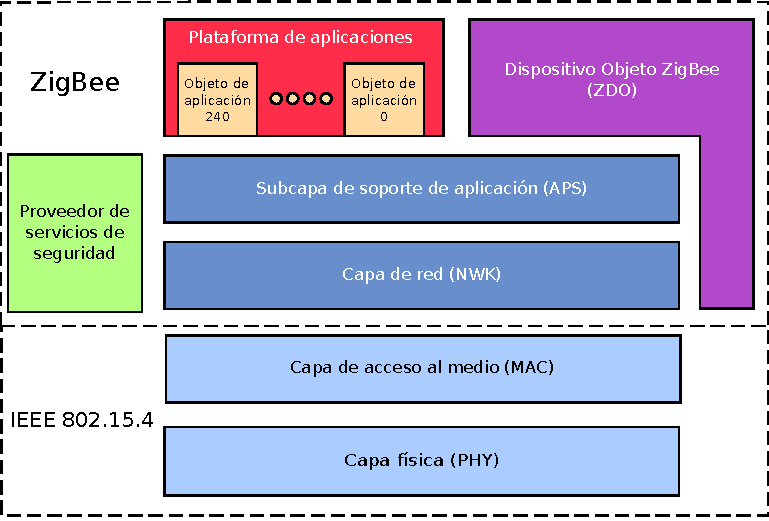
\includegraphics[scale=0.9]{capitulo_2_imgs/zigbee_arquitectura.pdf}
	\caption{Correlación de arquitecturas IEEE 802.15.4 y ZigBee}
	\label{img:ieee_zigbee}
\end{figure}

El estándar define dos tipos de dispositivos: 

\begin{itemize}
	\item Dispositivos de función completa (\textit{Full-Function Device}, FFD): Implementan todas las funciones de red, pueden comunicarse con cualquier otro dispositivo y funcionar como coordinador de la red, 
	\item Dispositivos de función reducida (\textit{Reduced Function Device}, RFD): Realiza funciones de red limitadas, sólo puede comunicarse con los FFD; se encarga de tareas simples como el sensado de variables del ambiente. 
\end{itemize}

La interacción entre FFD y RFD puede presentarse en dos topologías de red: Topología en estrella o topología punto a punto (o malla). En la topología en estrella un FFD opera como el coordinador de la red, mientras que los demás dispositivos, ya sean FFD o RFD, sólo pueden intercambiar información con el coordinador. En la topología punto a punto varios FFD pueden comunicarse entre sí, mientras que los RFD sólo pueden hacerlo con el coordinador de la red. Las topolog\'ias estrella y punto a punto se muestran en la figura \ref{img:ieee_topologia}.

\begin{figure}
	\centering
	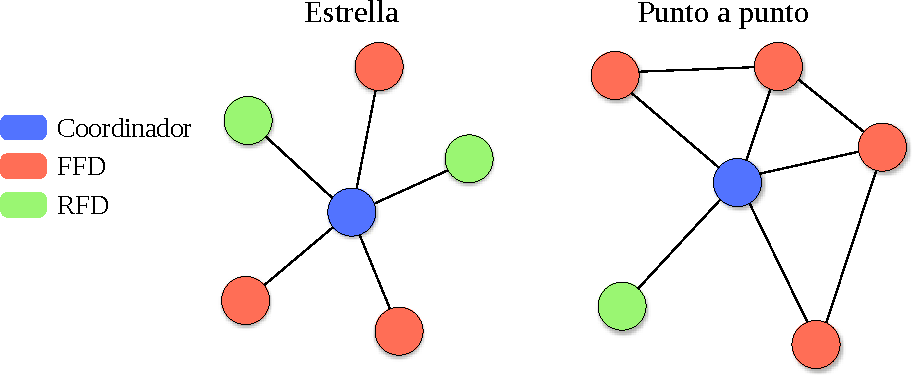
\includegraphics[scale=0.73]{capitulo_2_imgs/topologias_ieee80215.pdf}
	\caption{Topologías de red en el estándar IEEE 802.15.4.}
	\label{img:ieee_topologia}	
\end{figure}

Se definen dos tipos de acceso al medio: 1) acceso sincronizado y 2) acceso aleatorio. El acceso sincronizado se realiza cuando en una topología de estrella el coordinador de la red emite paquetes de datos periódicos para sincronizar la transferencia con los demás dispositivos. En el acceso aleatorio no existe sincronización de parte del coordinador de la red, este tipo de acceso se utiliza en la topología punto a punto. 

\subsubsection{ZigBee}

El estándar ZigBee define las capas superiores a IEEE 802.15.4 agregando funcionalidades de red, seguridad e interfaces de desarrollo para aplicaciones con LR-WPAN en dispositivos de bajo costo. Tiene como objetivo proveer conectividad inalámbrica auto organizable, reparable, de fácil instalación y mantenimiento optimizando el consumo de energía haciendo posible que los dispositivos puedan operar con baterías y de manera autónoma durante años.

La arquitectura de ZigBee, ver figura \ref{img:ieee_zigbee}, define dos capas principales: 1) la capa de red (NWK) y la capa de aplicaciones (APL). En la capa NWK se agrega la topología en malla, se determinan rutas de paquetes a través de la red e implementan comandos de seguridad. En esta capa se definen tres tipos de dispositivos: 

\begin{itemize}
	\item Coordinador ZigBee (CZ): Es el responsable de inicializar y controlar la red, establece las configuraciones iniciales de operación, asigna el canal de comunicación y el identificador único de la red; sólo puede existir un coordinador por cada red, 
	\item Router ZigBee (RZ): Se encarga de retransmitir información de otros dispositivos para establecer nuevas rutas o extender una red existente, 
	\item Dispositivo Final ZigBee (DFZ): Realiza operaciones de sensado y control, transmiten su información hacia los RZ o CZ. Puede entrar en modo de ahorro de energía interrumpiendo la comunicación inalámbrica en periodos preestablecidos. 
\end{itemize}
	
A diferencia de los DFZ, los CZ y RZ no pueden funcionar en modo de ahorro de energía, requieren operar en modo activo de manera permanente. 

En la configuración inicial de la red realizada por el CZ, se definen los parámetros de inicialización tales como la profundidad de la topología, niveles de seguridad y el número máximo de nodos hijos y routers. Se pueden formar topologías en árbol y malla, además de las disponibles en IEEE 802.15.4, ver figura \ref{fig:topologias_zigbee}. Con estas configuraciones de red es posible conectar con más de 64,000 nodos conectados a la misma red y, de esta manera, varios nodos CZ pueden interconectarse para formar redes más amplias.  

\begin{figure}
	\centering
	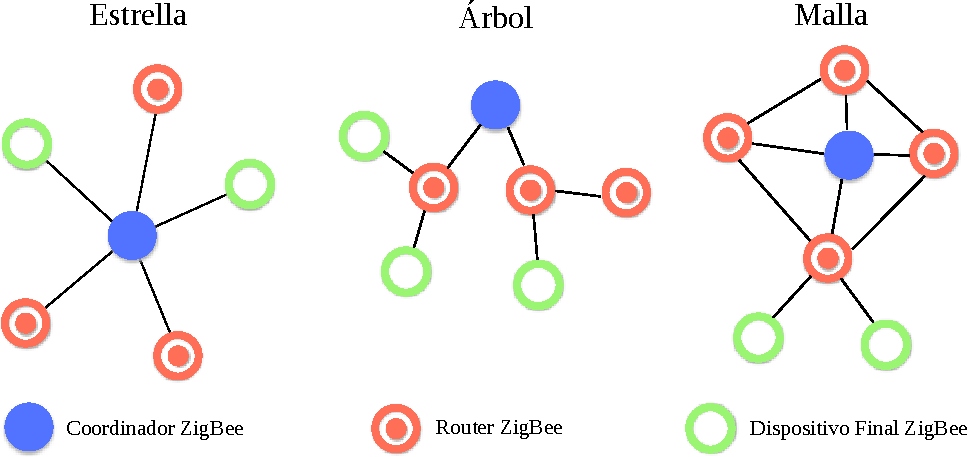
\includegraphics[scale=0.73]{capitulo_2_imgs/topologias_zigbee.pdf}
	\caption{Topologías de red en el estándar ZigBee}
	\label{fig:topologias_zigbee}
\end{figure}

APL es la capa más alta y sirve como interfaz entre el usuario y lo demás componentes de bajo nivel. Está formada de tres subcapas: 1) Plataforma de aplicaciones: Contiene las aplicaciones definidas por el usuario. Estas aplicaciones se separan en puntos finales (\textit{endpoints}), cada punto final encapsula algún comportamiento específico del dispositivo además de funcionalidades agregadas por el usuario, 2) Soporte de aplicaciones (APS): Actúa como un filtro entre la capa NWK y las aplicaciones. Se encarga de distinguir entre mensajes dirigidos a un punto final específico, y 3) Objetos de dispositivo ZigBee (ZDO): Se encarga de la administración de la red, provee servicios para encontrar otros nodos y servicios en la red, es responsable del estado actual del nodo en la red. 

\section{Sistemas de comunicaci\'on}

En esta aplicación se propone la conexión de la WSN con la estación remota via Internet, para ello se consideran dos escenarios de operación: 1) la instalación de la aplicación puede realizarse en zonas urbanas, y 2) la instalación de la aplicación en zonas rurales. Debido a esto, la selección de la tecnología utilizada para la comunicación remota de la WSN debe ser viable en ambos escenarios. 

Mediante \textit{Radio Módem} es posible transferir datos entre dos puntos con decenas de kilómetros de distancia con la posibilidad de incrementar este rango utilizando repetidores. Sin embargo, el costo del equipo e instalación es elevado, además de un alto consumo de energía. 

Por otro lado, la \textit{comunicación satelital} tiene una amplia cobertura aunque su disponiblidad depende de las condiciones climáticas; sus costos de instalación, mantenimiento y transmisión de datos son elevados. 

Para la comunicación remota entre la WSN y la estación base se requiere de un sistema de comunicación con amplia cobertura y bajo costo de mantenimiento. Por esta razón se propone utilizar el servicio GPRS. GPRS es un servicio de transmisión de datos vía radio que utiliza la red celular GSM (\textit{Global System for Mobile Communications}) para transferir datos mediante conmutación de paquetes. El servicio tiene una amplia cobertura y disponibilidad con un costo de transmisión por la cantidad de datos transmitidos. 

En la tabla \ref{tabla:tecnologias_com} se muestran las distintas tecnolog\'ias que se han mencionado para realizar la comunicación de una WSN con una estaci\'on base remota. Se puede ver que GPRS ofrece una amplia cobertura, sin embargo, el bajo costo de instalaci\'on, mantenimiento y transmisi\'on de datos respecto a las demás opciones es determinante en la selecci\'on de esta tecnolog\'ia.  


\begin{table}
	\begin{center}
		\caption{Tecnologías de comunicación}
		\label{tabla:tecnologias_com}
		\small
		\begin{tabular}{p{2cm}p{4cm}p{3.2cm}p{3.2cm}}
		\toprule
		\textbf{Tecnolog\'ia} & \textbf{Caracter\'isticas} & \textbf{Ventajas} & \textbf{Desventajas}\\
		\midrule
%		Bluetooth & Hasta 1 Mbps de velocidad de conexión hasta 10 m. & Altas velocidades de transmisión & Corto alcance y alto consumo de energía\\
		Enlace satelital & Comunicación de alta velocidad ideal para voz y video.  & Amplia cobertura, servicios disponibles con velocidad de transmisión de 10 Mbps. & Alto consumo de energía, alto costo de mantenimiento, susceptible a cambios en el clima.\\
		IEEE 802.11 & Comunicación entre dispositivos en rango 100 metros a gran velocidad. & Velocidad de transmisión de hasta 54 Mbps, bajo costo de instalación & Alto consumo de energía, cobertura limitada\\
		Radio módem & Comunicación digital mediante radio frecuencia & Velocidad de transmisión de 150 kbps, fácil implementación. & Alto costo de instalación y mantenimiento\\
		Red celular & Comunicación móvil a través de redes de comunicación celular GSM/GPRS & Amplia cobertura y altas velocidades de transmisión & El costo es proporcional a la cantidad de datos transmitidos \\
		Ethernet & Comunicación mediante redes de área local & Alta velocidad de transmisión & Corto alcance, requiere de infraestructura instalada\\
		\bottomrule
		\end{tabular}
	\end{center}
\end{table}

\subsection{La computadora industrial MOXA W315A}

En este proyecto se considera a la computadora embebida industrial MOXA W315A mostrada en la figura \ref{fig:moxa}. Este dispositivo integra un transceptor GSM/GPRS cuatribanda con interfaces de comunicación Ethernet y serial con un procesador ARM de 32 bits. Su diseño le permite operar en ambientes adversos con un amplio rango de temperatura y humedad, adem\'as de ser resistente a vibraciones y golpes. Está diseñada para aplicaciones máquina a máquina, monitoreo, conversión de protocolo y control. Sus características principales son: 

\begin{figure}
	\centering
	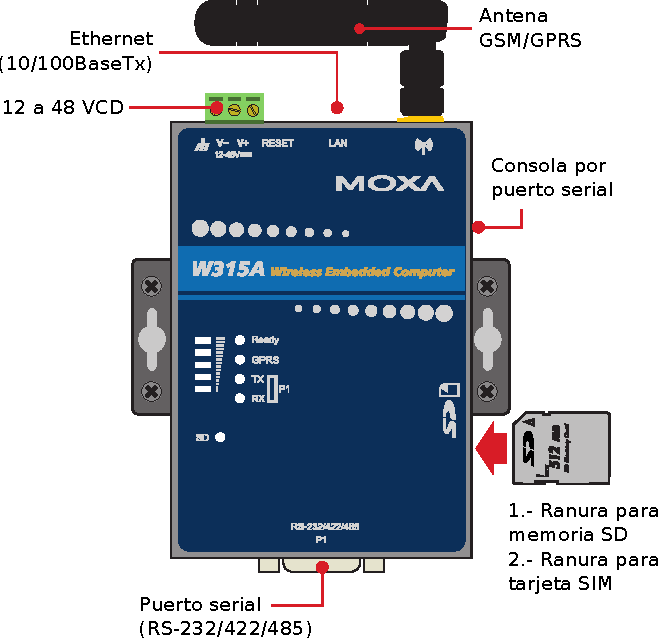
\includegraphics[scale=0.7]{capitulo_2_imgs/moxa.pdf}
	\caption{Computadora embebida industrial MOXA W315A}
	\label{fig:moxa}
\end{figure}

\begin{itemize}
	\item Procesador MOXA ART ARM9 32-bits de 192 MHz,
	\item 32 MB en RAM y 16 MB en memoria flash integrada, 
	\item Transceptor GSM/GPRS cuatribanda 850/900/1800/1900 MHz,
	\item Puerto serial RS-232/422/485 seleccionable por software, 
	\item Puerto Ethernet 10/100 Mbps,
	\item Ranura para memoria SD,
	\item Periféricos adicionales: RTC (\textit{Real Time Clock}), Buzzer y WDT (\textit{Watch Dog Timer}),
	\item Plataforma Linux (kernel 2.6.9),
	\item Rango de voltaje de operación:  12 -- 48 Vcd ,
	\item Consumo de corriente de 400 mA, 
	\item Temperatura de operaci\'on de -10$^{\circ}$ a 60$^{\circ}$ C, 
\end{itemize}

El módulo GSM/GPRS permite enviar y recibir mensajes de texto (SMS), seleccionar la frecuencia de operación y establecer conexiones GPRS. El kernel Linux 2.6.9 implementa diversos protocolos (TCP, UDP, ICMP, etc) que ofrecen una conexión transparente hacia Internet ya sea mediante la interfaz Ethernet o el módulo GSM/GPRS. Además en el sistema se incluyen herramientas de gestión y diagnóstico de la conexión GPRS, así como un API para el desarrollo de aplicaciones que soporta el control de los periféricos del dispositivo. 

\section{Los nodos Atmel RZRaven}

Los nodos Atmel RZRaven\cite{rel:raven} son dispositivos programables con una arquitectura abierta para el desarrollo de aplicaciones de redes inalámbricas ZigBee, ver figura \ref{fig:raven}. Existen dos tipos de dispositivos: 1) el nodo \textit{RZUSBSTICK} y 2) el nodo \textit{AVRRAVEN}. 

El nodo RZUSBSTICK es un dispositivo que sirve como interfaz entre la red inalámbrica y una computadora mediante un puerto USB. Está formado por un microcontrolador de 8 bits AT90USB1287 que controla la comunicación inalámbrica y la interfaz USB hacia la computadora. 

El nodo AVRRAVEN es un dispositivo compuesto por un transceptor inalámbrico de 2.4 GHz, dos microcontroladores de 8 bits de baja consumo, una pantalla LCD, un sensor de temperatura, botones de interfaz y puertos de expansión para conectar sensores u otros dispositivos. Un microcontrolador ATmega1284p gestiona la comunicación inalámbrica mientras que un microcontrolador ATmega3290p controla los periféricos del nodo. Este nodo funciona con dos baterías tipo botón o mediante una fuente de alimentación externa. La WSN propuesta en este proyecto se formará con nodos AVRRAVEN.

\begin{figure}
	\centering
	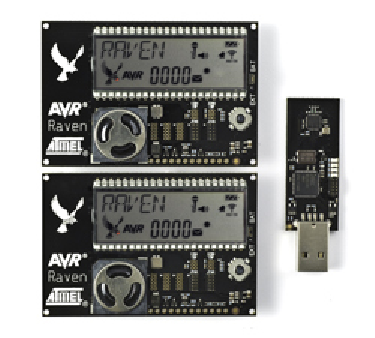
\includegraphics[scale=0.9]{capitulo_2_imgs/raven.pdf}
	\caption{Los nodos Atmel RZRaven}
	\label{fig:raven}
\end{figure}

\section{Atmel BitCloud}

Atmel BitCloud\cite{atmel:bitcloud} es una implementación en software de los estándares IEEE 802.15.4 y ZigBee que ofrece una pila de desarrollo multicapa con protocolos de comunicación y servicios compartidos de administración de tareas, configuración, seguridad y manejo de energía. El núcleo de la arquitectura de BitCloud, ver figura \ref{fig:bitcloud}, se basa en la definición de ZigBee con la subcapa de soporte de aplicación (APS) como interfaz entre las aplicaciones y capas inferiores de red (NWK) y acceso al medio (MAC). La capa de dispositivos ZigBee (ZDO) provee funciones de administración de red y comandos de búsqueda de servicios y dispositivos en la red. 

En el nivel más bajo de la arquitectura, la capa HAL (\textit{Hardware Abstraction Layer}) incluye un conjunto de funciones para el control de los distintos periféricos del microcontrolador (memoria EEPROM, temporizadores) e interfaces para la comunicación con dispositivos externos. La capa BSP (\textit{Board Support Package}) contiene manejadores para los periféricos disponibles en el dispositivo (sensores, memorias externas, botones). 

Los servicios compartidos, representados como capas verticales en la figura \ref{fig:bitcloud}, son responsables de 1) manejar los parámetros de configuración del dispositivo, 2) de la administración de tareas mediante la planificación del uso del CPU entre los componentes internos y la aplicación y 3) del control del consumo de energía administrando los ciclos de inactividad de los periféricos y conservando su estado de ejecución. Estos servicios compartidos están disponibles para las capas de todos los niveles de BitCloud.

\begin{figure}
	\centering 
	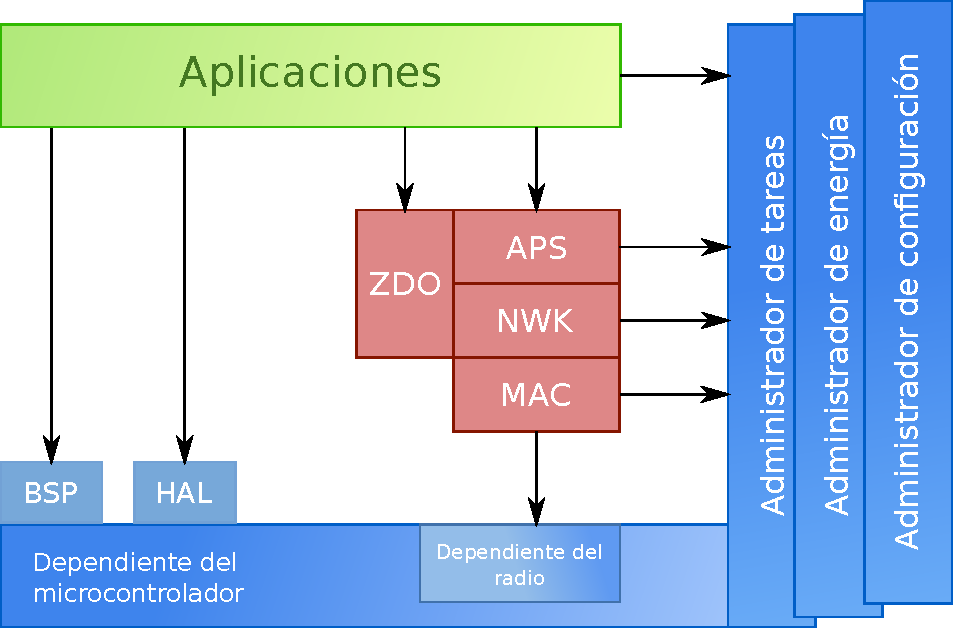
\includegraphics[scale=0.5]{capitulo_2_imgs/pila_bitcloud.pdf}
	\caption{Pila de desarrollo BitCloud}
	\label{fig:bitcloud}
\end{figure}

Distintas arquitecturas de hardware son soportadas en BitCloud, entre ellas los nodos RZRaven. Por esta razón, durante el desarrollo de este trabajo se utilizará a BitCloud para el desarrollo de la aplicación de la WSN. 
%\subsection{Programación orientada a eventos}

%La programación orientada a eventos es un paradigma de programación utilizado ampliamente en sistema embebidos donde los recursos de memoria y procesamiento son limitados. En este estilo de programación, cada función genera una señal asíncrona en cuanto termina su ejecución. Esta señal es entregada a través una llamada (\textit{Callback}) asociada a la función inicial. Es decir que al final de la ejecución de cada función, se ejecutará una función de respuesta. 

\subsection{Desarrollo de aplicaciones con Atmel BitCloud}

Cualquier aplicación de BitCloud debe ser considerada como otro elemento de la pila, esto implica que las aplicaciones deben utilizar los mismos mecanismos de interacción que los componentes internos. En BitCloud la mayoría de las funciones dentro de sus componentes se ejecutan de manera asíncrona, razón por la cual se utiliza comunicación solicitud/confirmación para pasar información entre las distintas capas. 

En este modelo de comunicación entre capas, cada función ejecutada recibe como uno de sus parámetros una función que será llamada una vez que haya terminado su ejecución. Asi mismo, es posible definir funciones que serán ejecutadas cuando se presenten eventos externos, como mensajes entrantes de la red inalámbrica o recibir señales eléctricas de algún sensor.   

Por otro lado, debido a que BitCloud está diseñado para ejecutarse en hardware con bajos recursos, la administración de tareas se realiza en un sólo hilo de ejecución, donde se determina la secuencia y prioridad de ejecución de las tareas de cada nivel de la pila. Para desarrollar aplicaciones dentro de este modelo de ejecución, el manual de programación de BitCloud recomienda representar a las aplicaciones como máquinas de estados finitos. 

Esta abstracción le permite al programador separar en bloques o estados a la lógica de la aplicación. Sin embargo, se deben considerar las siguientes restricciones para asegurar el correcto funcionamiento del administrador de tareas: 

\begin{itemize}
	\item Cada función que realice solicitudes a otros niveles de la pila debe definir una función de confirmación que será ejecutada una vez que se haya completado la solicitud inicial, 
	\item Es responsabilidad del usuario definir llamadas de confirmación para eventos inesperados tales como mensajes entrantes de la red inalámbrica, mensajes entrantes por la interfaz serial o interrupciones de señales eléctricas generadas por sensores u otros dispositivos,  
	\item El tiempo de ejecución de las funciones de confirmación no deben ser mayor a 10 ms, esto es para no interferir con las tareas de mayor prioridad en la pila. Si alguna función requiere mayor tiempo entonces se le puede asignar un estado dentro de la máquina de estados finitos de la aplicación, el cual será ejecutado una vez que el administrador de tareas le conceda la ejecución a la capa de aplicación, 
	\item Debido a que la capa de aplicación cuenta con la menor prioridad en la pila, la ejecución de funciones dentro de este nivel no debe ser mayor a 50 ms. Esto con la finalidad de no interferir con la ejecución de las funciones con una prioridad mayor. 
\end{itemize}


